\documentclass{article}%
\usepackage[T1]{fontenc}%
\usepackage[utf8]{inputenc}%
\usepackage{lmodern}%
\usepackage{textcomp}%
\usepackage{lastpage}%
\usepackage[head=40pt,margin=0.5in,bottom=0.6in]{geometry}%
\usepackage{graphicx}%
%
\title{\textbf{Protestan en la Universidad de los Llanos en rechazo a las nuevas tablas salariales}}%
\author{WALTER OBREGON}%
\date{18/09/2018}%
%
\begin{document}%
\normalsize%
\maketitle%
\textbf{URL: }%
http://www.eluniversal.com/venezuela/20999/protestan{-}en{-}la{-}universidad{-}de{-}los{-}llanos{-}en{-}rechazo{-}a{-}las{-}nuevas{-}tablas{-}salariales\newline%
%
\textbf{Periodico: }%
EU, %
ID: %
20999, %
Seccion: %
venezuela\newline%
%
\textbf{Palabras Claves: }%
NO\_TIENE\newline%
%
\textbf{Derecho: }%
2.3%
, Otros Derechos: %
NO\_TIENE%
, Sub Derechos: %
2.3.4%
\newline%
%
\textbf{EP: }%
SI\newline%
\newline%
%
\textbf{\textit{Se declararon en conflicto por considerar un descalabro lo que ha sufrido el salario de los profesores, empleados y obreros de dicha casa de estudios superiores}}%
\newline%
\newline%
%
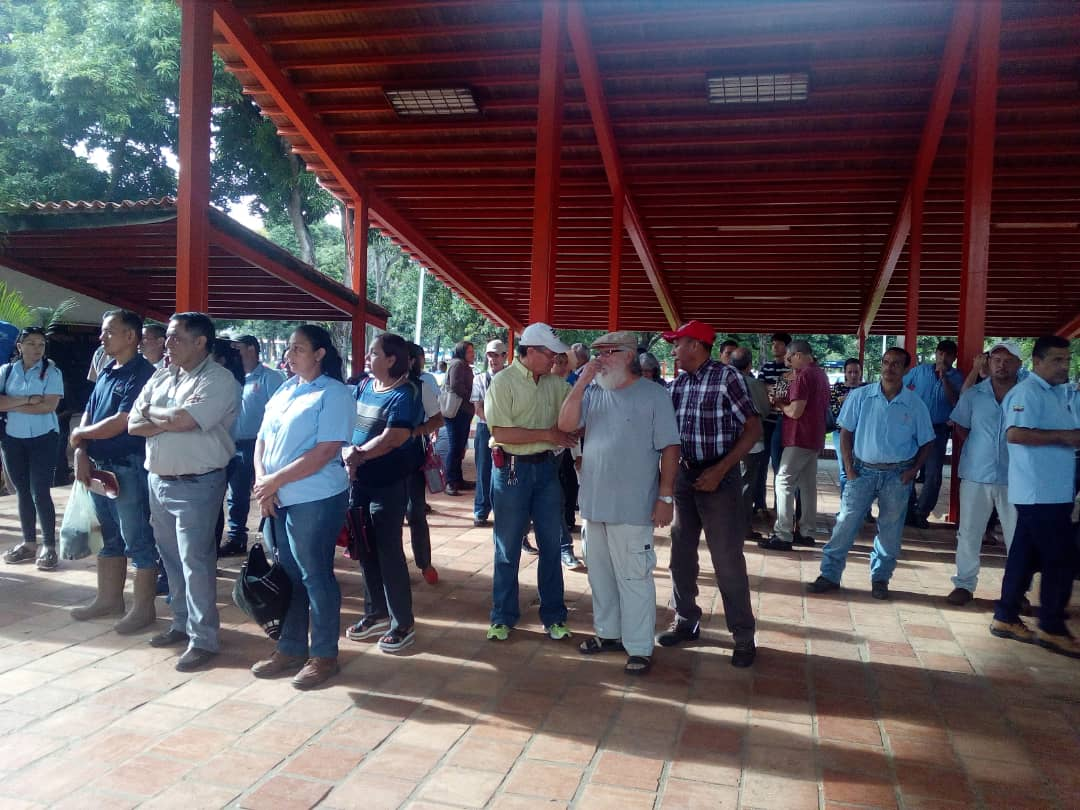
\includegraphics[width=300px]{171.jpg}%
\newline%
%
Barinas.{-} Este lunes los profesores, empleados y obreros de la Universidad de los Llanos Ezequiel Zamora (Unellez) de Barinas, protestaron pacíficamente en contra de las nuevas tablas salariales, que califican como una "imposición" del Ministerio para la Educación Universitaria Ciencia, Tecnología (Mppeuct).%
\newline%
%
Los afectados sostuvieron una asamblea en los espacios del rectorado unellista, donde lograron discutir la situación tomando decisiones que consideran pertinentes en esta lucha laboral.%
\newline%
%
José Felitas, vocero de los profesores (Apunellez), Brunilda Yánez de los empleados (Aeunellez) y el sindicalista Edelso Bastida (Sintraunellez), tomaron en consideración seis puntos a seguir como acciones de conflicto en la búsqueda de sus reivindicaciones.%
\newline%
%
Decidieron realizar paros escalonados a partir de la presente fecha, una nueva toma de la entrada principal el miércoles 19 de septiembre, sostener reuniones entre los tres gremios (Apunellez, Aeunellez y Sintraunellez) para constituir una asociación intergremial, convocar a otros sectores laborales de Barinas para una toma de la ciudad, incorporar a los estudiantes a la lucha y que los profesores informen a éstos la situación presentada para contar con su apoyo.%
\newline%
%
\end{document}